\section{Action Planning and Scheduling}\label{sec:plan}

The Gantt chart in chapter gives a brief overview of all tasks done for the project.
It lists important milestones and tasks along with information about who of the three team members\footnote{In this context, `St' stands for `Stefan', `Se' for `Sebastian' and `Bj' for `Björn'} is mainly involved.

Most defined deadlines could be reached in time.
Some tasks could even be started earlier than expected, particularly the testing of communication to the backend (due to consequent test-driven development) and the integration of the backend into Android app and NFC terminal ($\rightarrow$ continuous integration).

Since we lingered a bit too long with vain attempts to integrate our solution into Mr.~Recksiegel's hardware (c.f.~section \ref{sec:project_flow}) some tasks were slightly behind schedule.
These hardware problems also had effects on subsequent tasks.
Delayed tasks are marked with yellow and orange lines in the Gantt chart.


\iffalse
The chart includes tasks since the start of the project.
These already finished steps focused on conceptual and organisational aspects.
Most importantly, we obtained approval of important TUM stakeholders:
\begin{itemize}
\item Mr.~Bernhofer from the TUM IT Management, responsible for identity management and connections to external IT systems. He provided us with information how to access central TUM services (Active Directory, Token management for TUMonline, ...).
\item Mr.~Recksiegel from the TUM physics department, who is the head behind an existing student card to NFC solution running in the physics building. He promised help with hardware issues and to finally push the integration of our smartphone to NFC solution into the already existing systems.
\end{itemize}
%Mr.~Recksiegel also mentioned another possible field of application: 
%die Duschen halt....
\fi





%\newpage



\par\vfill\break % Break Last Page

\advance\vsize by 6cm % Advance page height
\advance\voffset by -2cm % Shift top margin
% Start big page
\centerline{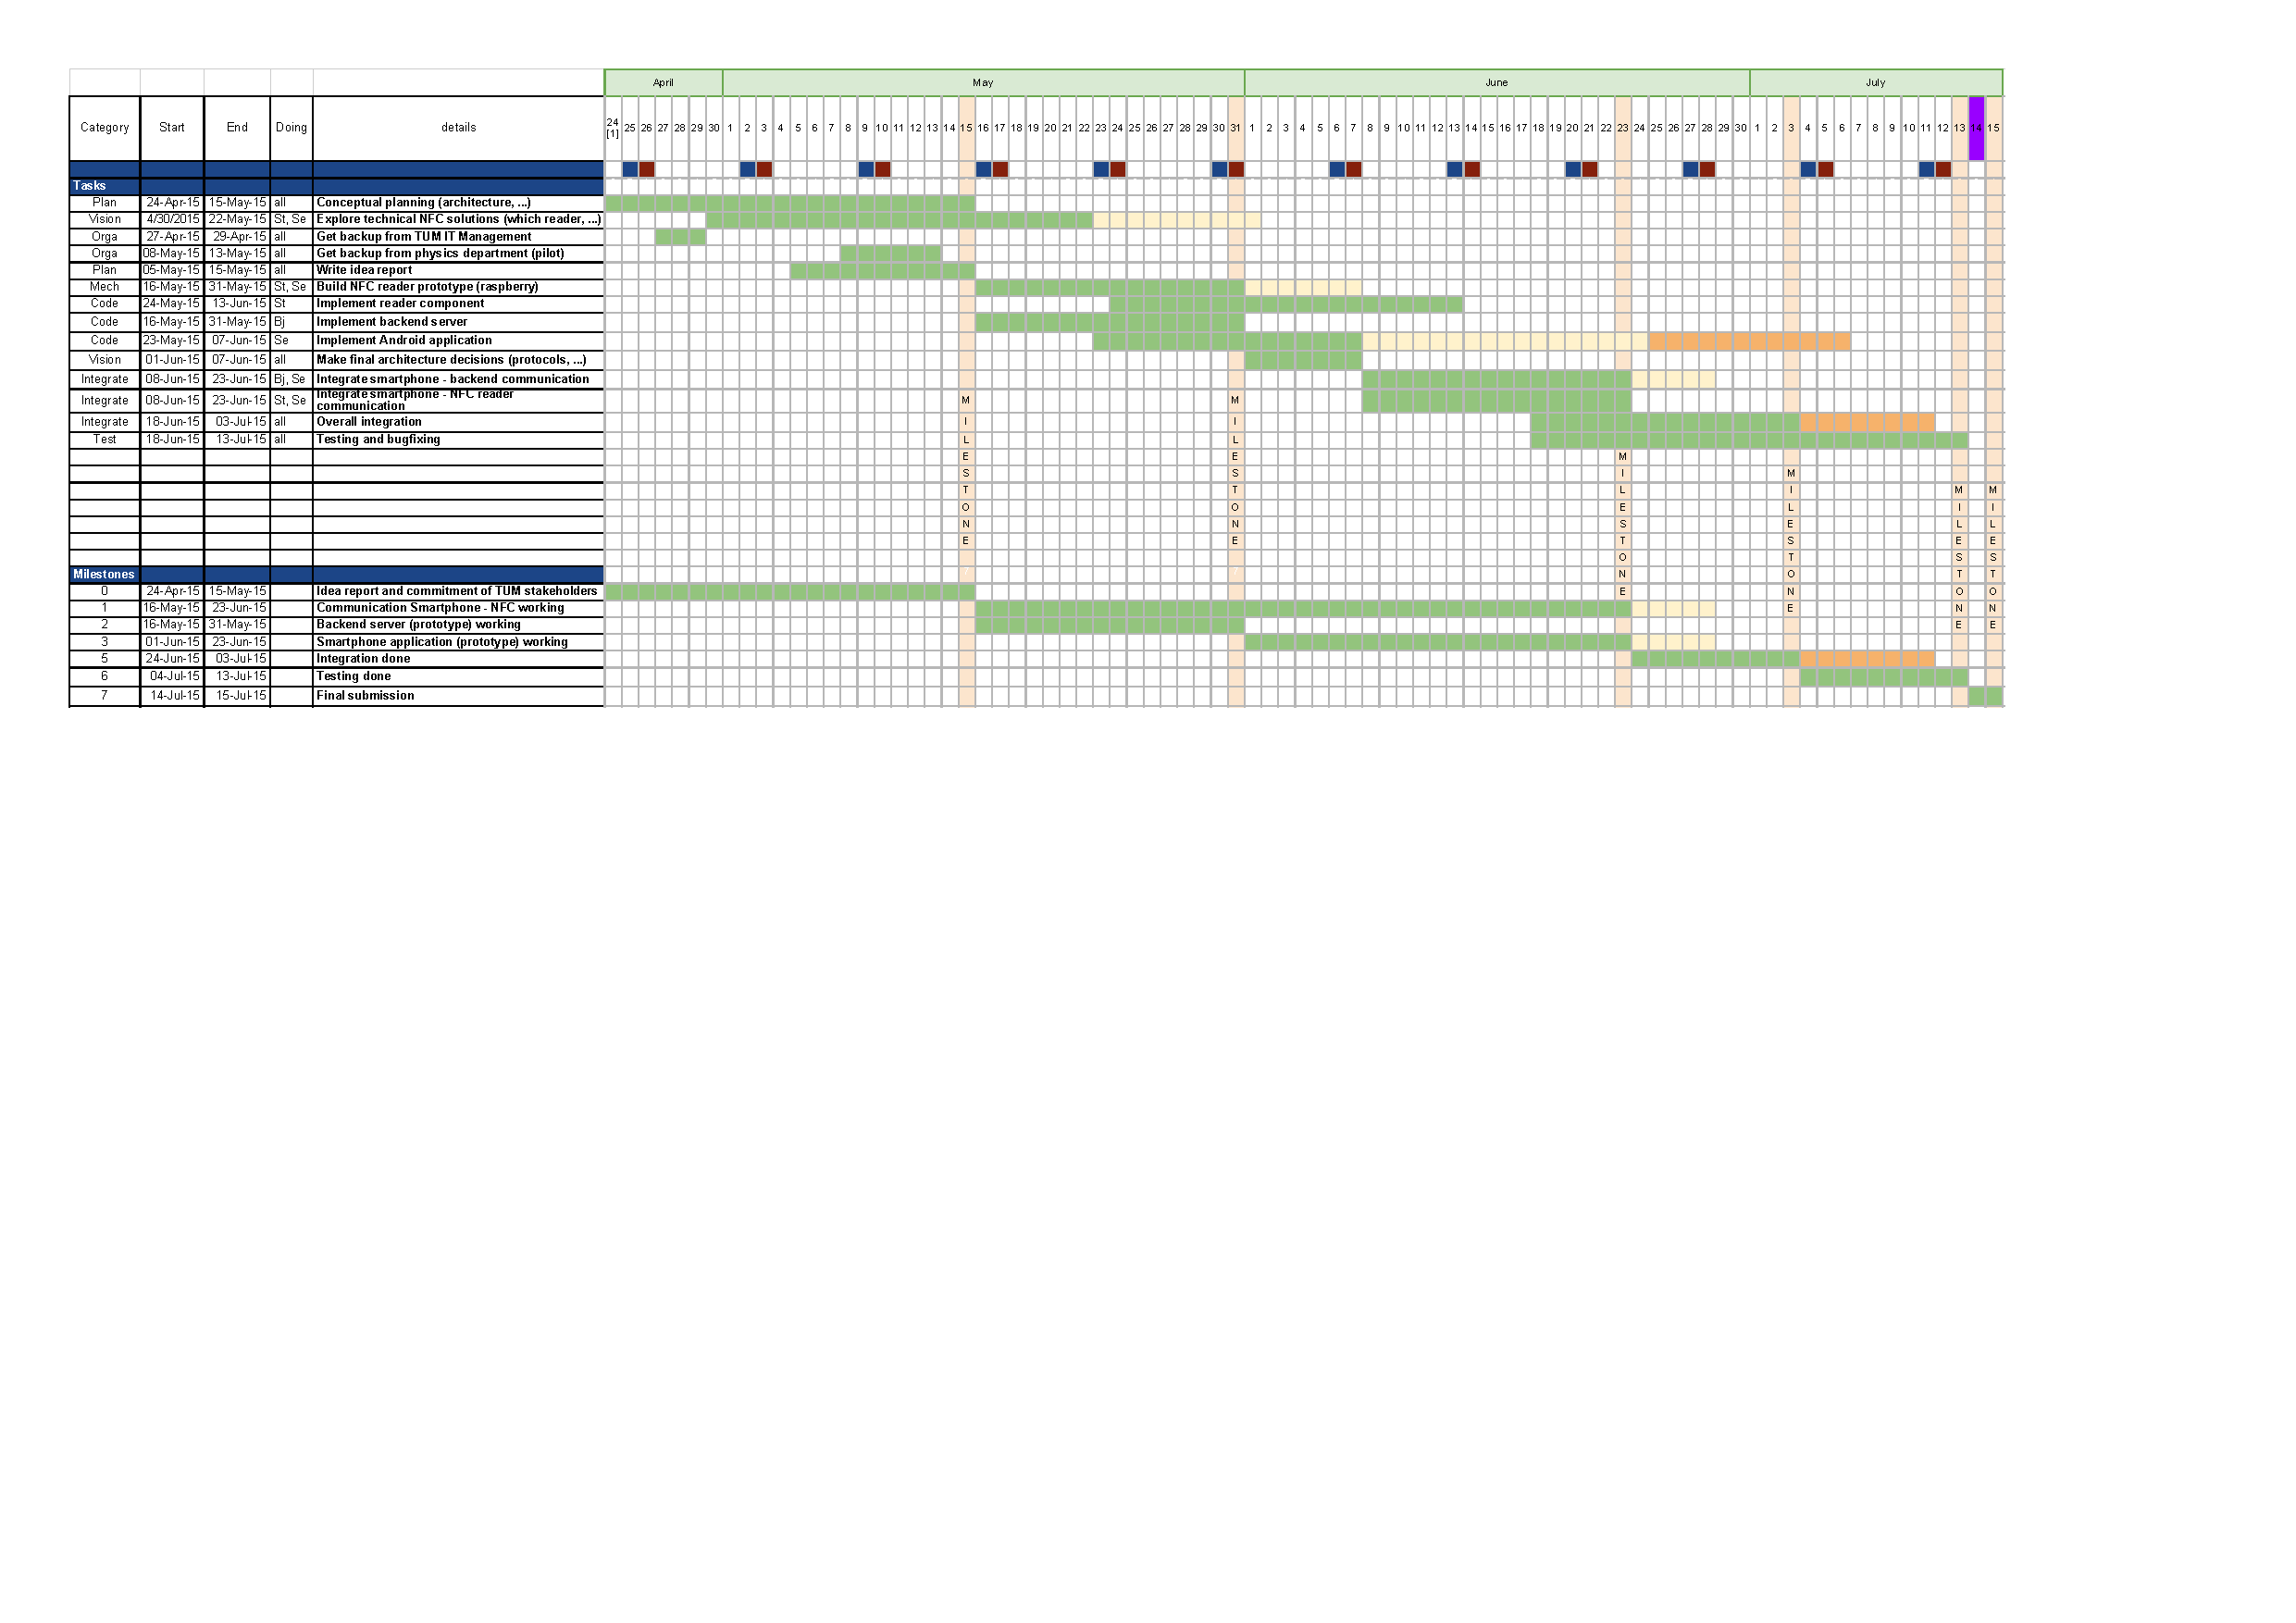
\includegraphics[height=79mm,angle=270]{gantt_final}}
% End big page
\par\vfill\break % Break the page with different margins

\advance\vsize by -6cm % Return old margings and page height
\advance\voffset by 2cm % Return old margings and page height